\documentclass{article}
\usepackage{geometry}
\geometry{a4paper, top=3cm, bottom=3cm, left=2cm, right=2cm}
\usepackage[utf8]{inputenc}
\usepackage[english]{babel}
\usepackage{hyperref}
\makeindex

\title{Foundations of Artificial Intelligence}
\author{Riccardo Salvalaggio}
\date{19th of April, 2021}

\usepackage{amssymb}
\usepackage{amsmath}
\usepackage{txfonts}
\usepackage{mathdots}
\usepackage{graphicx}

\begin{document}

\maketitle
\newpage
\tableofcontents
\newpage

\section{Introduction}
Artificial Intelligence is the attempt to make computers more "intelligent" to better understand human intelligence.
\section{Rational Agents}
It is a model that perceive the environment through sensors and act through actuators. In order to evaluate their performance use performance measure (e.g. vacuum -> level of cleanliness etc.) even if optimal behaviour is often unattainable because it is quite impossible to reach the goal in every aspect.\\ \textbf{Omniscent }if it knows the effects of its actions.\\ \textbf{Rational} agent behaves according to its percepts and knowledge and attempts to maximize the expected performance.\\ \textbf{Ideal: }for each possible percept sequence, selects an action that is expected to maximize its performance measure.
\subsection{Structure of Rational Agents}
The mapping is realised through an agent program executed on an Architecture which also provides an interface to the environment(percepts, actions)
\textbf{Agent = Architecture + Program}
\subsection{Classes of agents}
\subsubsection{Table-Driven (the simplest)}
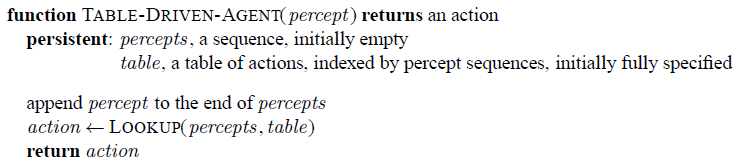
\includegraphics[scale=0.8]{1.png}\\
Problem: need a huge table to fulfill all the possible perceptions.\\

\subsubsection{Interpretative Reflex}
\begin{figure}[h!]
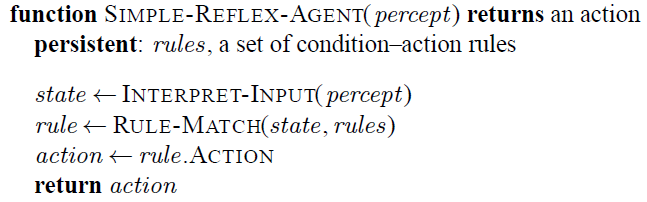
\includegraphics[scale=0.5]{2.png}
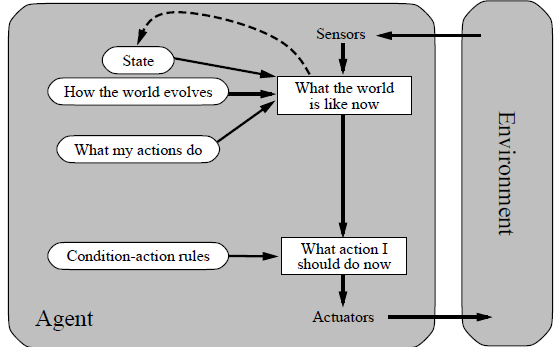
\includegraphics[scale=0.5]{3.png}\\
Interpretation of the input, matching to a rule to extract an action.
\end{figure}
\subsubsection{Model-Based Reflex}
\begin{figure}[h!]
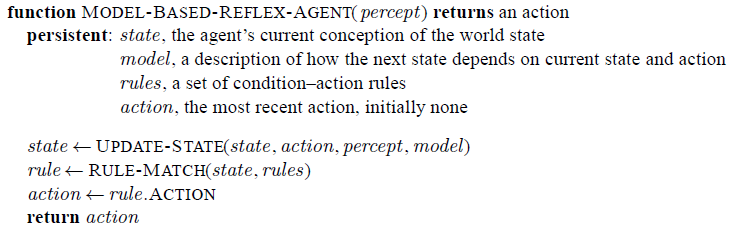
\includegraphics[scale=0.5]{4.png}
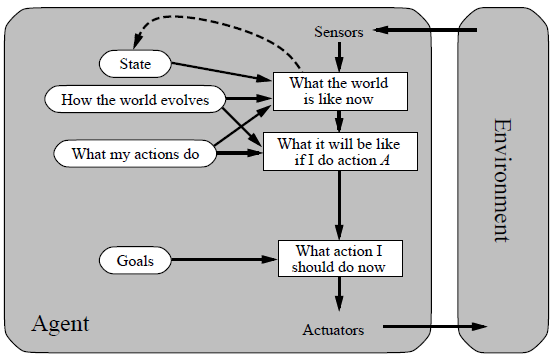
\includegraphics[scale=0.36]{5.png}
\caption{Goal-based}
\end{figure}
Introduction of a utlity function that maps a state onto a real number in order to compute the best action to do and to weigh the importance of competing goals.
\begin{figure}[h!]
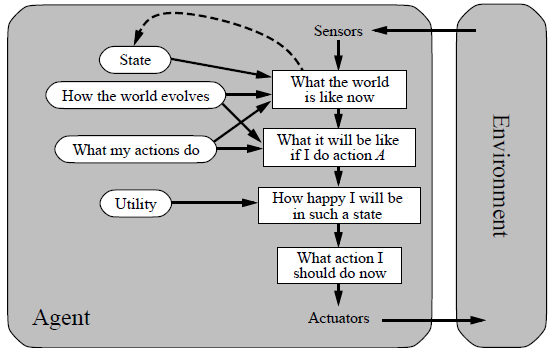
\includegraphics[scale=0.5]{6.png}
\caption{Utility-based}
\end{figure}
\subsubsection{Learning agents}
Agents that improve over time starting from an empty knowledge and unknown environments.\\
\textbf{Components: }\\
\textit{Learning element:} responsible for making improvements.\\
\textit{Performance element:} select external actions.\\
\textit{Critic: }determines performance of the agent.\\
\textit{Problem generator: }suggests actions that lead to informative experiences.\\
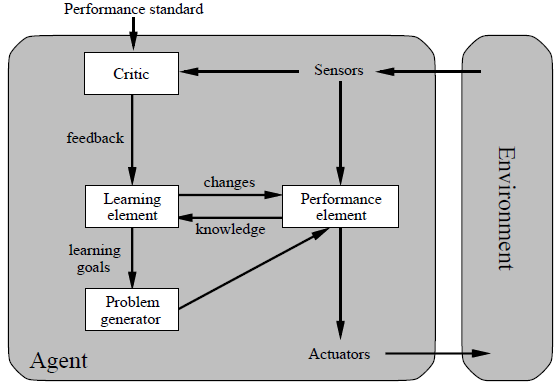
\includegraphics[scale=0.5]{7.png}
\subsection{Types of environments}
Accessible vs. inaccessible, Deterministic vs. stochastic, Episodic vs. sequential, static vs. dynamic, discrete vs. continuous, single vs. multi agent.

\section{Solving Poblems by Searching}
\subsection{Problem-solving agents}
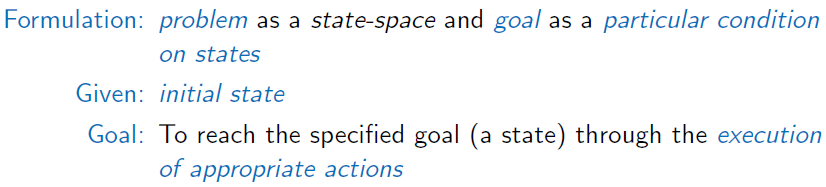
\includegraphics[scale=0.6]{8.png}\\
\begin{figure}
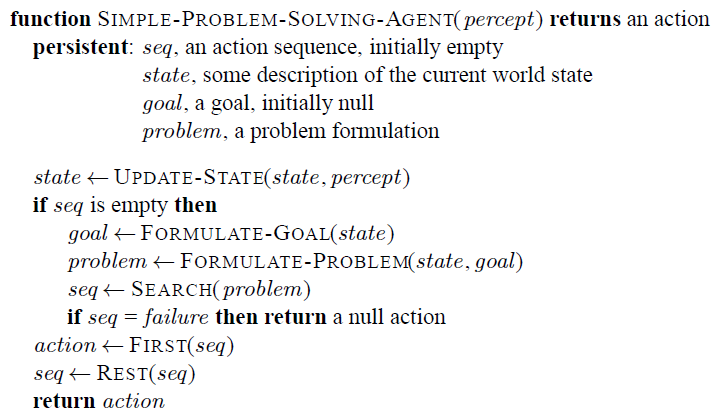
\includegraphics[scale=0.6]{9.png}\\
\caption{Simple Problem-solving Agent}
\end{figure}\\\\
- Properties: Fully-observable, Deterministic/static env., discrete states, single-agent.\\

\subsection{Problem Formulation}
Goal formulation, definition of: State space, actions, problem type, search and execution costs.\\
\subsection{Problem Types}
Based on knowledge of States and Actions: Observability, completeness of knowledge about world state and actions. (e.g. If the environment is completely observable, the vacuum cleaner always knows where it is and where the dirt is.)\\
Transition Model: Description of the outcome of an action.\\
Solution: Path from the initial to a goal state.\\
Search Costs: Time and storage requirements to and a solution.\\
Total Costs: Search costs + path costs.\\
Alternative formulations can influence a lot number of states, e.g. 8 queens problem: Naive - billions of state, Better - 2057 states.\\
Examples of Real-World Problems: Route planning, shortest path problem, TSP, VLSI Layout, Robot nav., Assembly sequencing.\\
\subsection{Search strategies}
E.g.: node expansion, frontier, search strategy, tree-based search, graph-based search.\\
- Search Tree Data structure:\\
state, parent, action, path-cost.\\

\begin{figure}[h!]
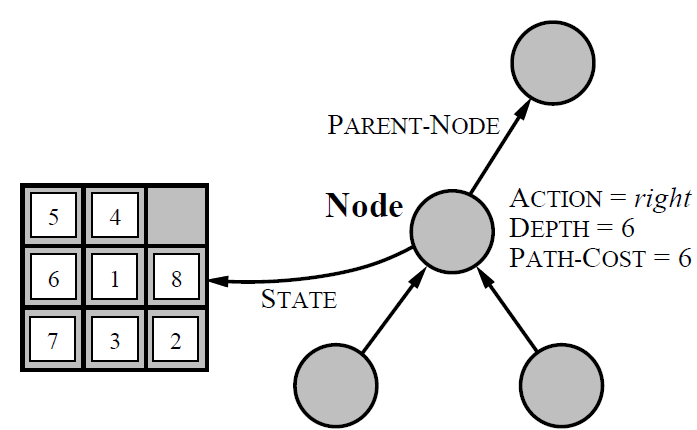
\includegraphics[scale=0.6]{10.png}
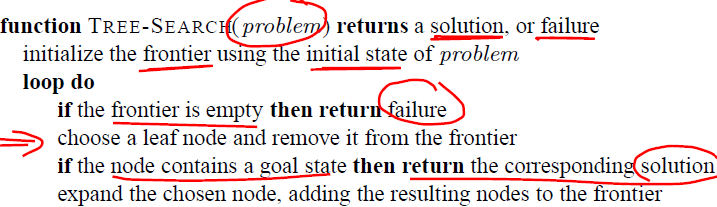
\includegraphics[scale=0.6]{11.png}
\end{figure}

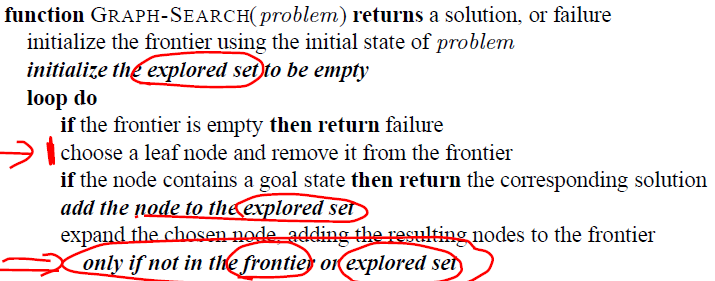
\includegraphics[scale=0.6]{12.png}\\\\
- Criteria for Search Strategies: \textbf{\textit{Completeness, Time complexity, Space Complexity, Optimality}}.\\

\subsubsection{Uninformed or blind searches}
- Breadth-First Search:\\
Nodes are expanded in the order they were produced (first siblings, then children) (frontier = FIFO queue). Completeness is obvious, the solution is optimal. \textbf{Time complexity: }Let b be the maximal branching factor and d the depth of a solution path. Then the maximal number of nodes expanded is = O(b at d).\textbf{ Space Complexity: O(b at d)}\\\\
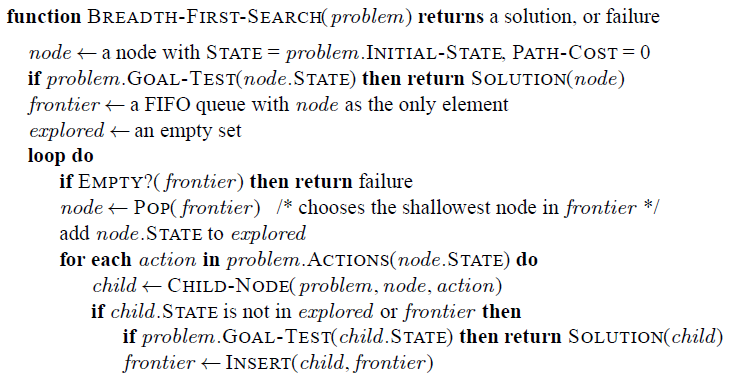
\includegraphics[scale=0.6]{13.png}\\\\
- Uniform-Cost Search:\\
If step costs are different, uniform cost is better. It expands node with lowest path costs \textit{g(n)}. It uses a Priority queue. Always finds the cheapest solution, given that g(successor(n)) $>=$ g(n) for all n.\\
- Depth-First Search:\\
Always expands an unexpanded node at the greatest depth (frontier $<-$ a LIFO queue, first children, then siblings). Usually implemented recursively.\\
Generally, optimal is not guaranteed. Completeness only for graph-based search. \textbf{Time complexity: }in graph-based is bounded by the space, so it can be infinite, in tree-based: O(b at m) (m max length of a path). \textbf{Space Complexity: }tree-based: O(b*m), graph-based: worst-case, all states need to be stored. (no better than breadth-first).\\\\
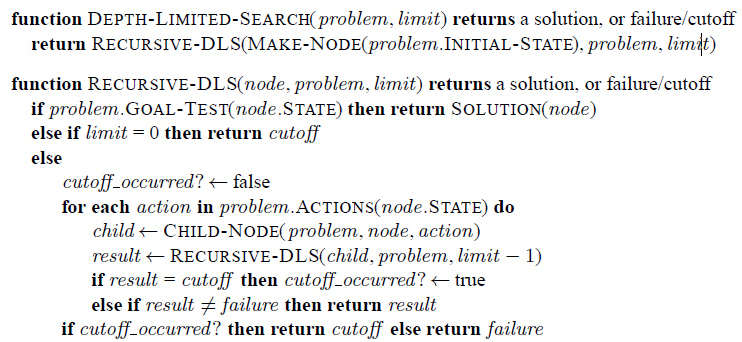
\includegraphics[scale=0.6]{14.png}\\\\
- Iterative Deepening Search:\\
Like depth-limited search and in every iteration increase search depth by one. Combines depth and breadth-first. Optimal and complete like breadth-first, but requires much less memory: O(b*d).\\\\
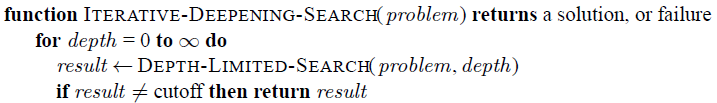
\includegraphics[scale=0.6]{15.png}\\\\
Iterative deepening in general is the preferred uninformed search method when there is a large search space and the depth of the solution is not known.\\
For small space it is worse than breadth-fist.\\
- Bidirectional searches:\\
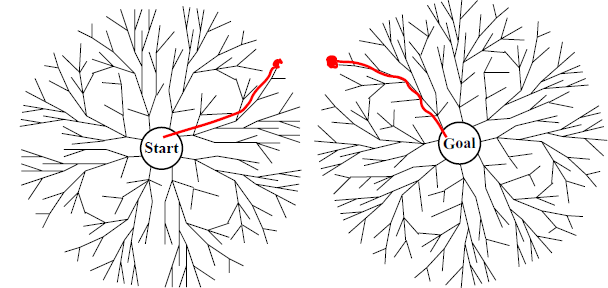
\includegraphics[scale=0.6]{16.png}\\\\
As long as forward and backward searches are symmetric, search times of O(2*b at d/2) = O(b at d/2) can be obtained. The operators are not always reversible, there must be an efficient way to check if a new node already appears in the search tree of the other half of the search.\\
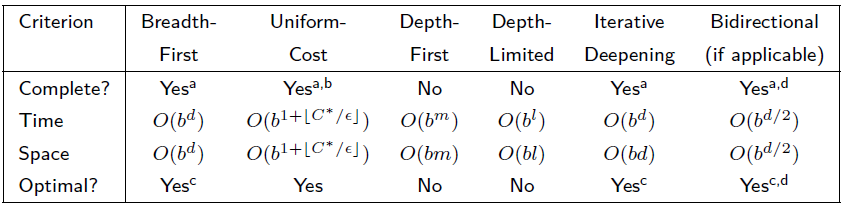
\includegraphics[scale=0.6]{17.png}

\section{Informed Search Methods}
- Uninformed: rigid procedure with no knowledge of the cost of a given node to the goal.\\
- Informed: knowledge of the worth of expanding a node n is given in the form of an evaluation function f(n) which assigns a real number to each node. Mostly,
f(n) includes as a component a heuristic function h(n), which estimates the costs of the cheapest path from n to the goal.\\
- Best-first: informed that expands with the best f-value.\\\\
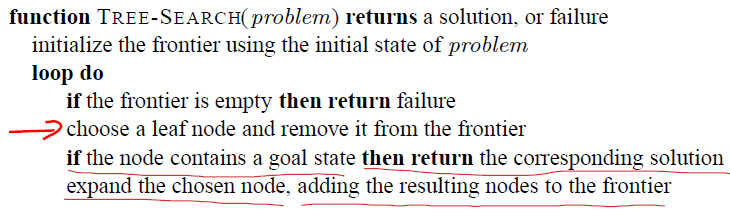
\includegraphics[scale=0.6]{18.png}
Instance of tree-search algorithm in which frontier is a priority queue. When f is always correct, we don't need to search.\\
\subsection{Greedy Search}
h(n) = estimated path-costs from n to the goal. A best-first search using h(n) (heuristic function) as evaluation function is called greedy search.
\subsection{Heuristics}
Heuristics are fast but in certain situations incomplete methods for problem-solving, they improve the search in the average-case and the time complexity. In general, not optimal and incomplete; graph-search version is complete only in finite spaces.
\subsection{A* and IDA*}
A* combines greedy search with the uniform-cost search: always expand node with lowest f(n) = g(n) (actual cost from start to n) + h(n) (estimated cost to goal/optimistic estimate of the costs). A new h is \textit{admissible} iff: h(n) $<=$ h*(n).
\subsubsection{Optimality of A*}
\textbf{Claim: }The first solution found has the minimum path cost.\\
\textbf{Proof: }Suppose there exists a goal node G with optimal path cost f*, but
A* has first found another node G2 with g(G2) > f*. Let n be a node on the path from the start to G that has not yet been expanded. Since h is admissible, we have: f(n)$<=$f* $-->$ f(G2)$<=$f(n) $-->$ f(G2)$<=$f* $==>$ g(G2)$<=$f* Contraddiciton.\\
- Completeness: If a solution exists, A* will find it provided that (1) every node has a finite number of successor nodes, and (2) there exists a positive constant $\delta$ > 0 such that every step has at least cost $\delta$.\\
- Complexity: In general, still exponential in the path length of the solution (space, time), it depends on the choice of Heuristic used.
\subsubsection{Graph- vs. Tree-search}
For the graph-based variant, either needs to consider re-opening nodes from the explored set, when a better estimate becomes known, or needs to require stronger restrictions on the heuristic estimate: it needs to be consistent (iff for all actions a leading from s to s': h(s) - h(s') $<=$ c(a), where c(a) denotes the cost of action a). Consistency implies admissibility, A* can still be applied if heuristic is not consistent but optimality is lost.
\subsubsection{Variants of A*}
In general suffers from exponential memory growth.
- Iterative-deepening A*: f-costs are used to define the cut-off (IDA*).\\
- Recursive Best First Search (RBFS): introduces a variable \textit{f-limit} to
keep track of the best alternative path, if the limit is exceeded opt for the alternative path.\\
- MA* and SMA*.

\subsection{Local Search Methods}
In many problems we are interested only to solving it, not how. If there is also a quality measure, local search can be used.\\
It uses a Hill Climbing/ Gradient descent mechanisms (improvements step by step), requires few memory because it operates using just the current node.\\\\
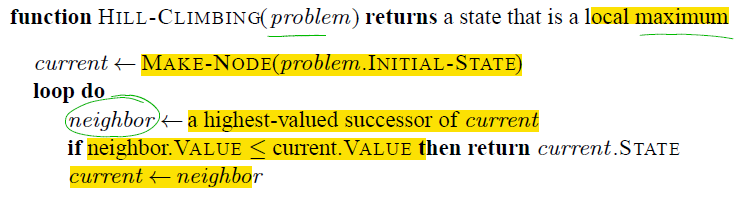
\includegraphics[scale=0.6]{19.png}\\\\
- Problem: the algorithm can stop in a sub-optimal solution (local maxima), the algorithm explore at random (plateaus), requires also suboptimal moves (ridges).\\
- Solution: restart if no improvements, inject noise.\\\\
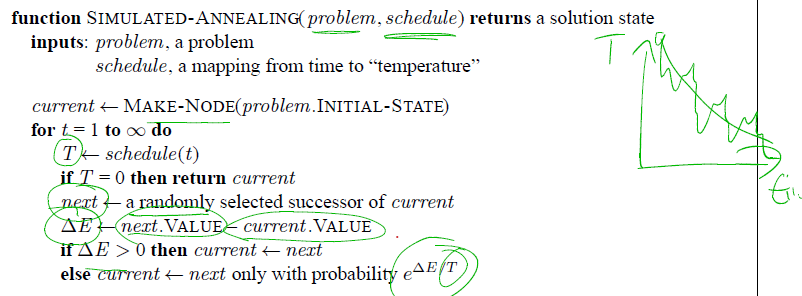
\includegraphics[scale=0.6]{20.png}

\subsection{Genetic Algorithms}
Similar to evolution, we search for solutions by three operators: "mutation","crossover", and "selection". Need of coding a solution into a string of symbols or bit-string, fitness function to judge the worth of configurations.\\Example: Represent an individual (one 8-queens configuration) as a concatenation of eight x-y coordinates. Its fitness is judged by the number of non-attacks. The population consists of a set of configurations.\\

\section{Board games}
The states of a game are easy to represent. The possible actions of the players are well-defined.\\
The game can be implemented as a kind of search problem, the individual states are fully accessible and is nonetheless a contingency problem, because the actions of the opponent are not under the control of the player.\\
Board games are not only difficult because they are contingency problems, but also because the state space can become astronomically large.\\
\subsection{Minimax search}
In contrast to regular searches, where a path from beginning to end is a solution, max must come up with a strategy to reach a favorable terminal state regardless of what min does $->$ all of min moves must be considered and reactions to them must be computed.\\
When it is possible to produce the full game tree, the minimax algorithm delivers an optimal strategy for max.\\
- Algorithm:\\
1. Generate the complete tree with depth-first search.\\
2. Apply utility function.\\
3. Determine the utility: if predecessor is MIN, assign minimum value, if predecessor is MAX, assign maximum value.
Predecessor node is a max-node: Value is the maximum of its child nodes
From the initial state (root of the game tree), max chooses the move that
leads to the highest value (minimax decision).\\\\
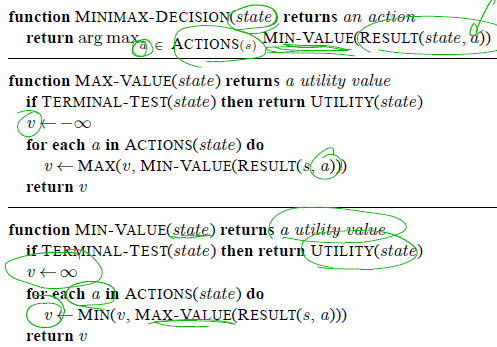
\includegraphics[scale=0.6]{21.png}

\subsection{Alpha-Beta Search}
When the tree is becoming too large, we have to evaluate correctly where to expand it. The design of the evaluation function is fundamental!\\
Standard evaluation functions are weighted linear
- Alpha-Beta pruning: $\alpha$ : value of the best choice for MAX, $\beta$ : value of the best choice for MIN.\\
(1) Prune below the min node whose $\beta$ -bound is less than or equal to the $\alpha$ -bound of its max-predecessor node.
(2) Prune below the max node whose $\alpha$ -bound is greater than or equal to the $\beta$ -bound of its min-predecessor node.\\\\
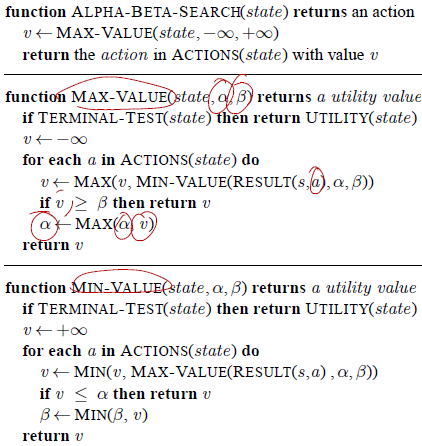
\includegraphics[scale=0.6]{22.png}\\\\
The alpha-beta search cuts the largest amount off the tree when we examine the best move first. Best case: O(b at d/2). Average case: O(b at 3d/4).Practical case: A simple ordering heuristic brings the performance close to the best case.\\
\subsection{Games with an Element of Chance}
In addition to min- and max nodes, we need chance nodes (e.g. for the dice).\\
\begin{figure}
	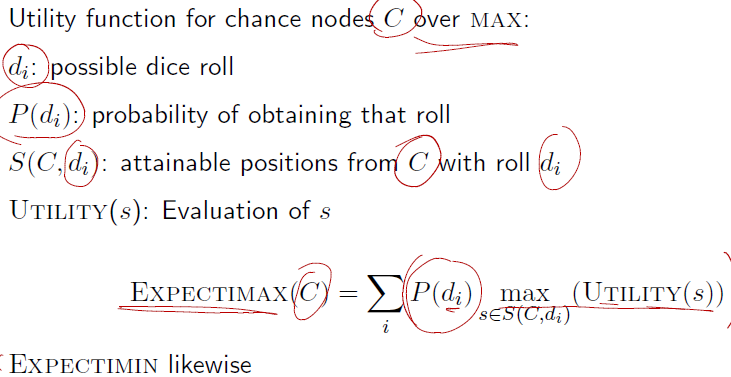
\includegraphics[scale=0.6]{23.png}
	\caption{Expected value}
\end{figure}
Search costs increase: Instead of O(b at d), we get O((b x n)at d), where n is
the number of possible dice outcomes.\\

\section{Constraint satisfaction problems}
Such problem is defined by:\\
- variables, a set of value domains, a set of constraints, an assignment.\\
Main idea is to exploit the constraints to delete large portions of search space.\\
A constraint graph can be used to visualize binary constraints, Nodes = variables, arcs = constraints.\\
State: a variable assignment.
\subsection{Backtracking search for CSPs}
It assigns values to variables step by step using DFS single-variable (Backtracing search).\\
\begin{figure}[h!]
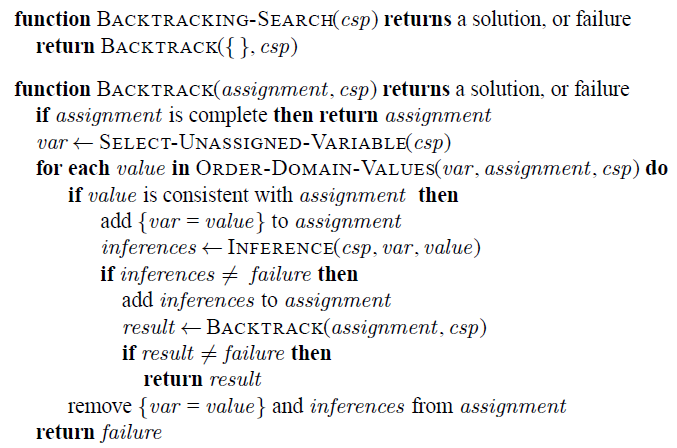
\includegraphics[scale=0.6]{24.png}
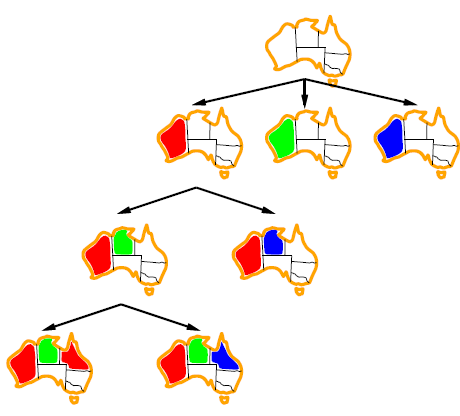
\includegraphics[scale=0.6]{25.png}
\end{figure}
\subsection{CSP Heuristics}
- Variable ordering: e.g.: most constrained first: choose the variable with the fewest remaining legal value.\\
- Value ordering: e.g.: Least constraining value first
- Rule out failures early: e.g. Forward checking:\\\\
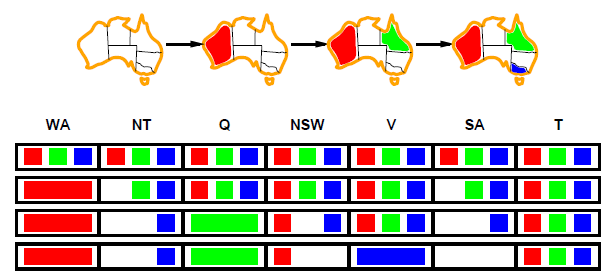
\includegraphics[scale=0.6]{26.png}
\subsection{Constraint Propagation}
A problem of Forward Checking is that constraints of unassigned variables are not propagated.\\
A directed arc X $->$ Y is consistent iff for every choice of x there exists y that satisfies constraints; It detects failures earlier, can be used as preprocessing.\\\\
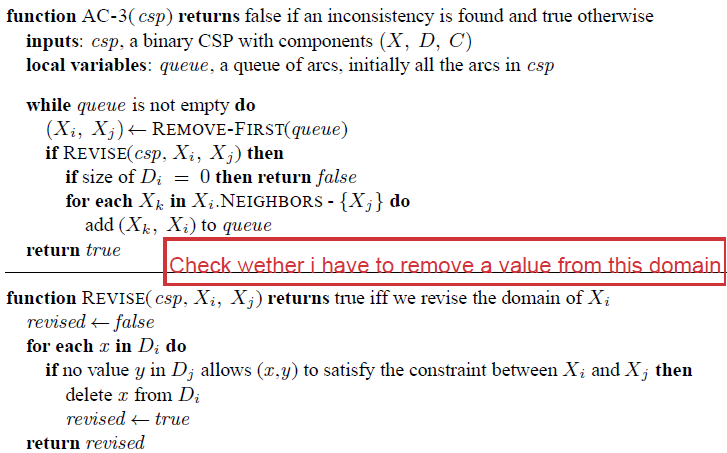
\includegraphics[scale=0.6]{27.png}\\\\
Time complexity: O(\[d^3 * n^2)\]). Of course, AC-3 does not detect all inconsistencies (which is an NP-hard problem).
\subsection{Problem Structure}
If the CSP graph is a tree, then it can be solved in O(\[nd^2\]) (general
CSPs need in the worst case O(\[d^n\] )). Pick root, order nodes, apply arc consistency bottom-up, assign starting at root. This algorithm is linear in n.\\
Another solution is to reduce the graph structure by fixing values in a reasonably chosen subset. Instantiate a variable and prune values in neighboring variables (\textbf{conditioning}).\\
Almost Tree construction:\\
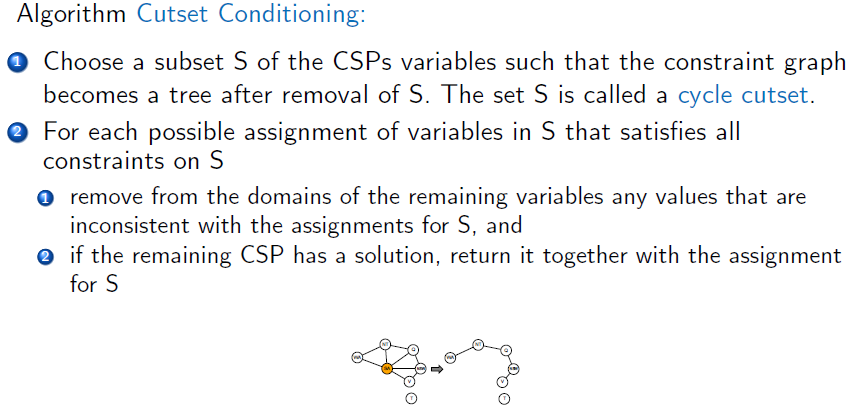
\includegraphics[scale=0.6]{28.png}\\\\
\textbf{- Tree Decomposition: }\\
Decompose the problem into a set of connected (\textit{share a constraint}) sub-problems and solve them independently. If a variable appears in two sub-problems, it must appear in all sub-problems on the path between the two sub-problems.\\
Consider sub-problems as new mega-variables, use tree-structured CSP to find solution.\\
The tree width w of a tree decomposition is the size of largest sub-problem minus 1, If a graph has tree width w and we know a tree decomposition with that width, we can solve the problem in O(\[nd^(w+1)\]).\\    

\section{Propositional logic}
Logic is a universal tool with many powerful applications.\\
\subsection{Agents that Think Rationally}
Rational action requires rational (logical) thought on the agent's part so they must know a portion of the world in its near (\textbf{Knowledge base, KB}). KB is compose of sentences in a logic language.\\
\textbf{- Levels: }\\
\textit{1. Knowledge level: }most abstract level, concerns the total knowledge.\\
\textit{2. Logical level: }encoding of knowledge in a formal language.\\
\textit{3. Implementation level: }the internal representation of the sentences. (as a string or as a value).\\\\
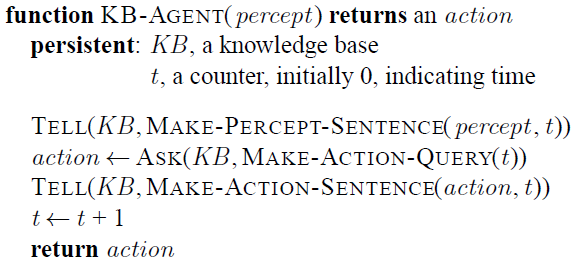
\includegraphics[scale=0.6]{29.png}\\\\
A logic also defines the semantics or meaning of sentences, defines the truth of a sentence with respect to each possible world. If a sentence $\alpha$ is true in a possible world m, we say that m satisfies $\alpha$ or m is a model of $\alpha$.\\
\textbf{- Logical entailment: }$\alpha$ |= $\beta$ iff in every model in which $\alpha$ is true, $\beta$ is also true. (follow from KB) e.g.: x = 0 $|=$ xy = 0.\\
\textbf{- Inference: }we can derive $\alpha$ with an inference method i. This is written as: KB |- $\alpha$. (Derivation)\\
\textbf{- Declarative Languages: }we state what we want to compute, not how. System believes P iff it consider P true. We must know symbols, when a sentence is true etc.\\
We'd like to have inference algorithms that derive only sentences that are entailed (\textit{soundness}) and \textbf{all} of them (\textit{completeness}).
The building blocks of propositional logic are indivisible, atomic statements.\\
\subsubsection{Syntax}
An Interpretation I is called model of $\omega$ if I $|=$ $\omega$.
A truth assignment of the atoms in $\Sigma$ , or an interpretation I over $\Sigma$ , is a function: I:$\Sigma$ $->$ {T,F}.\\
A formula $\phi$ can be: satisfiable, unsatisfiable, falsifiable (there exists I that doesn't satisfy $\omega$), valid (tautology: I $|= \omega$ $\forall$ I ), logically equivalent (I$|=\omega$ iff I$|=\chi$ $\forall$I). A method to decide if a formula is satisfiable is: Truth Table.
\subsubsection{Normal forms}
\textbf{- conjunctive normal form (CNF): }conjunction of disjunctions:\\
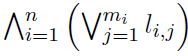
\includegraphics[scale=0.6]{30.png}\\
\textbf{- disjunctive normal form (DNF): }disjunction of conjunctions:\\
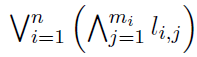
\includegraphics[scale=0.6]{31.png}\\
It is always possible to transform a formula in a CNF/DNF but the conversion can make the sentence growing in an exponential way.\\
\textbf{Some properties of logical implication: }\\
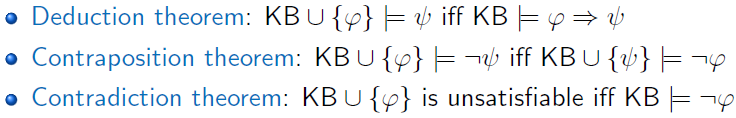
\includegraphics[scale=0.6]{32.png}\\\\
We can often derive new formulae from formulae in the KB. These new formulae should follow logically from the syntactical structure of the KB formulae.\\
\textbf{Calculus:} Set of inference rules (potentially including so-called logical axioms). A calculus C is sound (or correct) if all formulae that are derivable from a KB actually follow logically. A calculus is complete if every formula that follows logically from the KB is also derivable with C from the KB.\\
\textbf{Resolution}\\
We want a way to derive new formulae that does not depend on testing every interpretation (idea: to prove that KB $|=\phi$, we can prove that KB $\bigcup${$\neg \phi$} is unsatisfiable (contradiction theorem)).\\\\
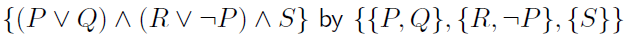
\includegraphics[scale=0.6]{34.png}\\
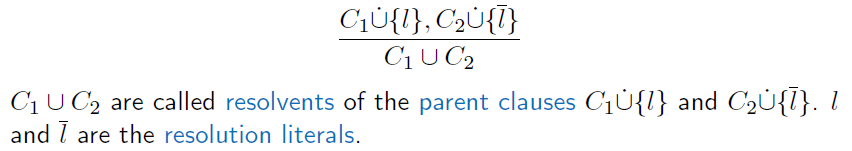
\includegraphics[scale=0.6]{35.png}\\
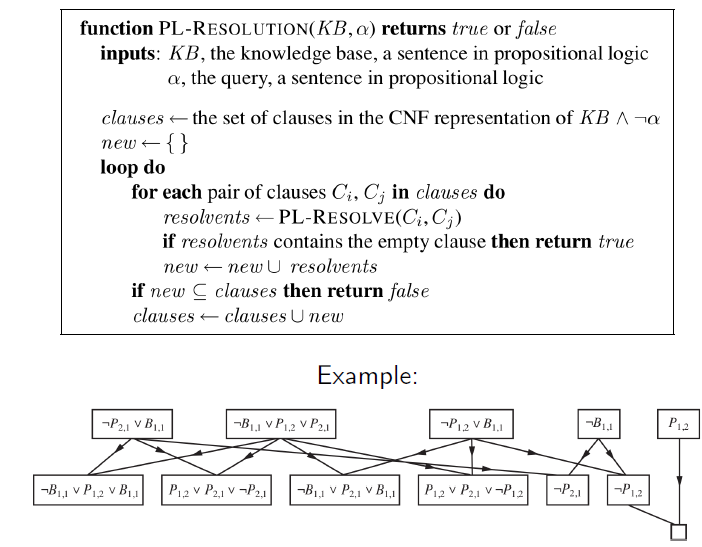
\includegraphics[scale=0.8]{33.png}\\\\
\textbf{Lemma (soundness)} If $\Delta |-$ D, then $\Delta |=$ D.\\
\textbf{Proof idea:} Since all D $\in$ R($\Delta$) follow logically from $\Delta$, the Lemma results through induction over the length of the derivation.\\
Is resolution also complete? So the opposite implications are also valid. Not in general.\\
However, it can be shown that resolution is refutation-complete: $\Delta$ is
unsatisfiable implies $\Delta |-$ empty.\\
\textbf{Theorem:} $\Delta$ is unsatisfiable iff $\Delta |-$ empty.\\\\
We can now infer new facts, but how do we translate knowledge into action?\\
\textbf{Negative selection: }Excludes any provably dangerous actions.\\
A1,1 $\wedge$ EastA $\wedge$ W2,1 $=> \neg$Forward\\
\textbf{Positive selection: }Only suggests actions that are provably safe.\\
A1,1 $\wedge$ EastA $\wedge$ $\neg$W2,1 $=> $Forward\\\\

\section{Satisfiability and Model Construction}
\textbf{SAT} solving is the best available technology for practical solutions to many NP-hard problems. Differently from Logical deduction, SAT returns a model of the theory (solution) given a logical theory. SAT can be formulated as a Constraint-Satisfaction-Problem ($->$ search):\\
\begin{itemize}
\item CSP-variables: alphabet\\
\item Domain: {True, False}\\
\item Constraints given by clauses\\
\end{itemize}
\subsection{Davis-Putnam-Logemann-Loveland (DPLL) Procedure}
It corresponds to backtracking with inference in CSPs. Inference in DPLL:\\
Simplify: if variable v is assigned a value d, then all clauses containing v
are simplied immediately (corresponds to forward checking), variables in unit clauses are immediately assigned.\\
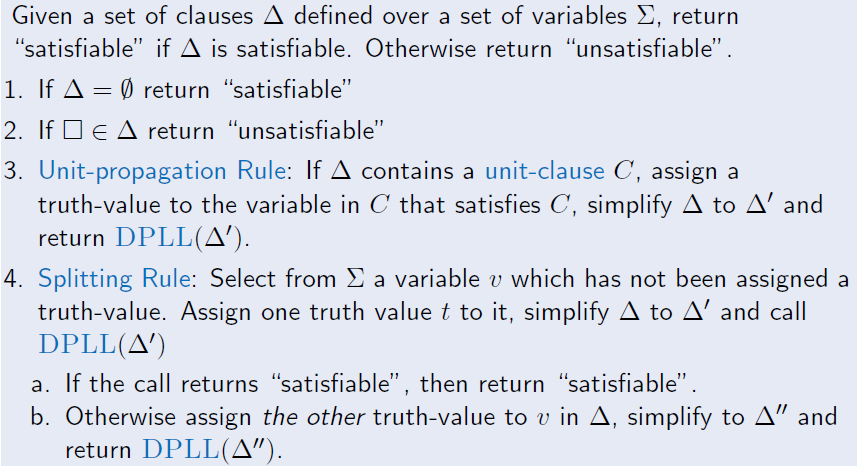
\includegraphics[scale=0.6]{36.png}\\
DPLL is complete, correct, and guaranteed to terminate. DPLL constructs a model, if one exists. In general, DPLL requires exponential time (splitting rule!), Heuristics are needed. DPLL is polynomial on Horn clauses. Horn Clauses constitute an important special case, since they require only polynomial runtime of DPLL. A \textbf{Horn clause }is a clause with maximally one positive literal.\\
\subsubsection{DPLL on Horn Clauses}
\begin{itemize}
\item \textbf{1.} The simplifications in DPLL on Horn clauses always generate Horn clauses
\item \textbf{2.} If unit propagation rule in DPLL does not lead to termination, a set of Horn clauses without unit clauses is generated.
\item \textbf{3.} A set of Horn clauses without unit clauses and without the empty clause is satisfiable, since: \\
\textit{All clauses have at least one negative literal.\\
Assigning false to all variables satisfies formula.}\\
\item \textbf{4.} It follows from 3.:
\begin{itemize}
\item a. every time the splitting rule is applied, the current formula is
satisfiable.\\
\item b. every time, when the wrong decision is made, this will be immediately detected.
\end{itemize}
\item \textbf{5.} Therefore, the search trees for n variables can only contain a maximum of n nodes, in which the splitting rule is applied (and the tree branches).
\item \textbf{6.} Therefore, the size of the search tree is only polynomial in n and therefore the running time is also polynomial.
\end{itemize}
For CNF-formulae, in which the probability for a positive appearance, negative appearance and non-appearance in a clause is 1/3, DPLL needs on average quadratic time. All NP-complete problems have at least one order parameter and the hard
to solve problems are around a critical value of this order parameter. This
critical value (a phase transition) separates one region from another, such as
over-constrained and under-constrained regions of the problem space.\\
\begin{figure}[bht!]
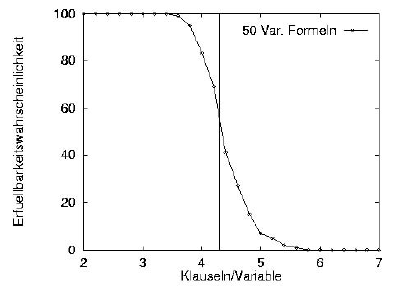
\includegraphics[scale=0.7]{37.png}
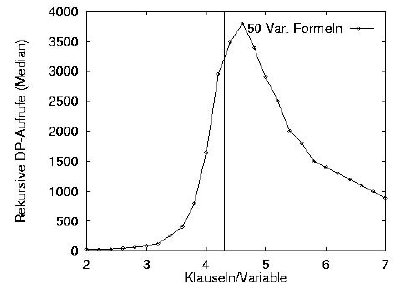
\includegraphics[scale=0.7]{38.png}
\end{figure}
When the probability of a solution is close to 1 \textbf{(under-constrained)}, there are many solutions. If the probability of a solution is close to 0 \textbf{(over-constrained)}.\\
\subsection{Local Search}
In many cases, we can sacrifice completeness if we can "solve" much larger instances this way. Standard process for optimization problems: \textbf{Local Search}. Problem: local minima. However: By restarting and/or injecting noise, we can often escape local maxima. Local search can perform very well for SAT solving.\\\\
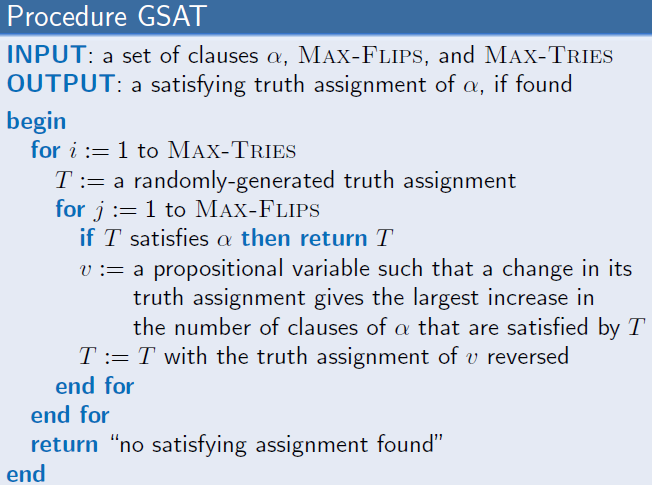
\includegraphics[scale=0.6]{39.png}\\\\
   
\subsection{State of the Art}
\subsubsection{Improvements of DPLL Algorithms}
Branching on variables can cause stopping, we can "learn" \textbf{(here: logically infer)} a new clause (negation of a variable). Leads to conflict-directed clause learning (CDCL).\\
Both for DPLL/CDCL algorithms and local search algorithms\\
\begin{itemize}
\item Randomization and restarts
\item Efficient data structures and indexing
\item Engineering ingenious heuristics
\end{itemize}
Meta-algorithmic advances\\
\begin{itemize}
\item Automated parameter tuning and algorithm configuration
\item Selection of the best-fitting algorithm based on instance characteristics
\item Selection of the best-fitting parameters based on instance characteristics
\item Use of machine learning to pinpoint what factors most affects performance.
\end{itemize}
\subsubsection{Algorithm configuration}
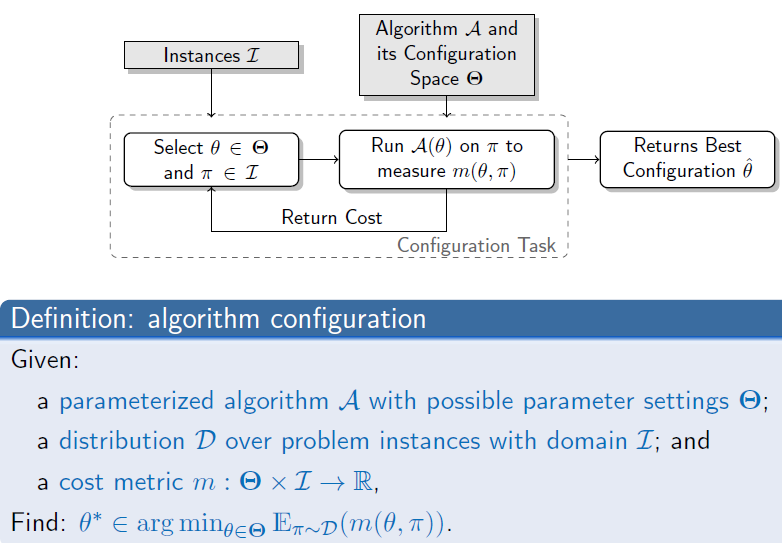
\includegraphics[scale=0.7]{40.png}\\
\textbf{- Strength: } find a single configuration with strong performance for a
given cost metric.\\
\textbf{- Weakness: }for heterogeneous instance sets, there is often no configuration that performs great for all instances.\\
\subsubsection{Algorithm selection}
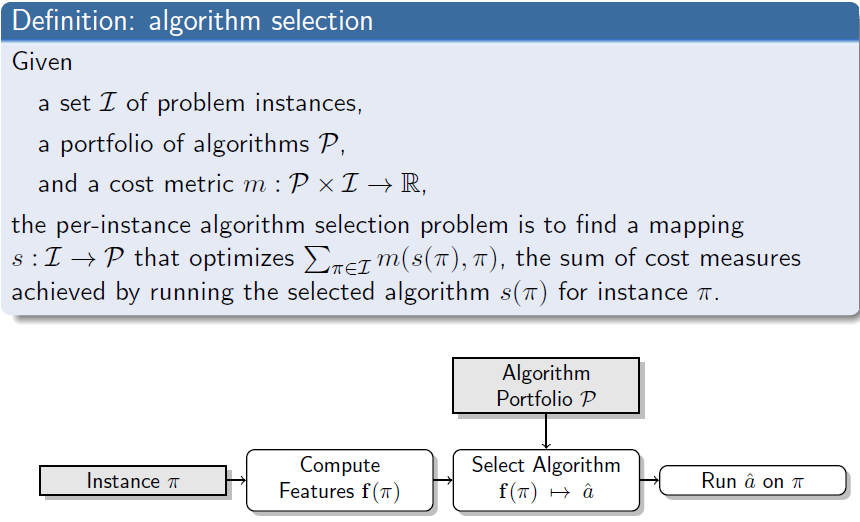
\includegraphics[scale=0.7]{41.png}\\
\textbf{- Strength: }for heterogeneous instance sets, pick the right algorithm
from a set.
\textbf{- Weakness: }the set to choose from typically only contains a few algorithms.
\subsubsection{Automated construction of portfolios from a single algorithm}
\textbf{Putting the two together: }Use algorithm configuration to determine useful configurations. Use algorithm selection to select from them based on instance
characteristics.\\\\
\textbf{Hydra}\\\\
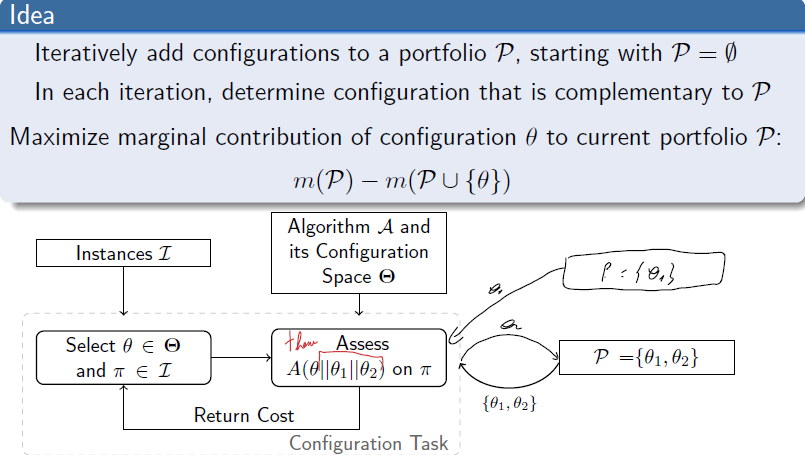
\includegraphics[scale=0.8]{42.png}

\section{Predicate Logic (First-Order Predicate Logic (PL-1))}
Propositional logic has no structure in the atomic propositions.\\
In addition to Operators, Variables, Brackets we have Predicate and function. They have an arity (number of arguments): 0-ary predicate: propositional logic atoms, 0-ary function = constants.\\ 
\textbf{Terms: }Every variable is a term, If t1, t2,..., tn are terms and f is an n-ary function, then f(t1, t2,..., tn) is also a term. Terms without variables: ground terms.\\
\textbf{Atomic Formulae: }Represent statements about objects.
\begin{itemize}
\item If t1, t2,...,tn are terms and P is an n-ary predicate, then P(t1, t2,...,tn) is an atomic formula.
\item If t1 and t2 are terms, then t1 = t2 is an atomic formula. Atomic formulae without variables: ground atoms (contain only ground terms). 
\end{itemize}
\subsection{Semantics of PL1-Logic}
\textbf{Interpretation: }I = <D,$x^I$> D domain, $x^I$ is a function that:\\
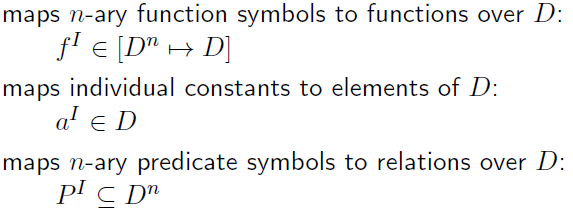
\includegraphics[scale=0.6]{43.png}\\
\textbf{Interpretation of ground terms: }$(f(t1,..., tn))^I$ = $f^I(t^I_1,...,t^I_n).$\\
\textbf{Satisfaction of ground atoms P(t1,...,tn): }I $|=$ P(t1,...,tn) iff <$t^I_1,..., t^I_n \in P^I$.
\subsubsection{Variable assignment}
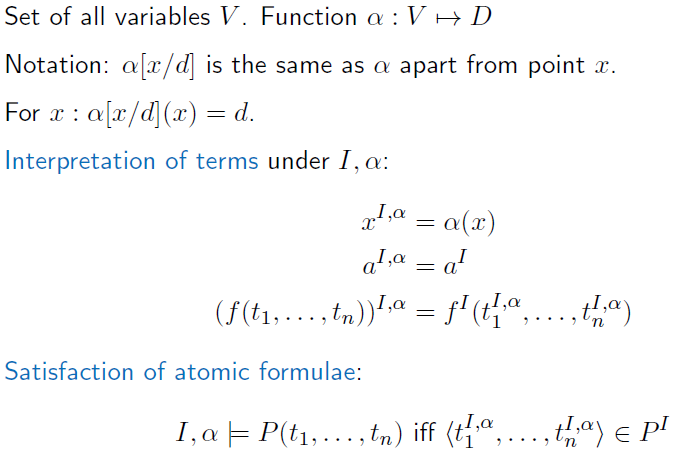
\includegraphics[scale=0.6]{44.png}
\subsubsection{Satisfiability}
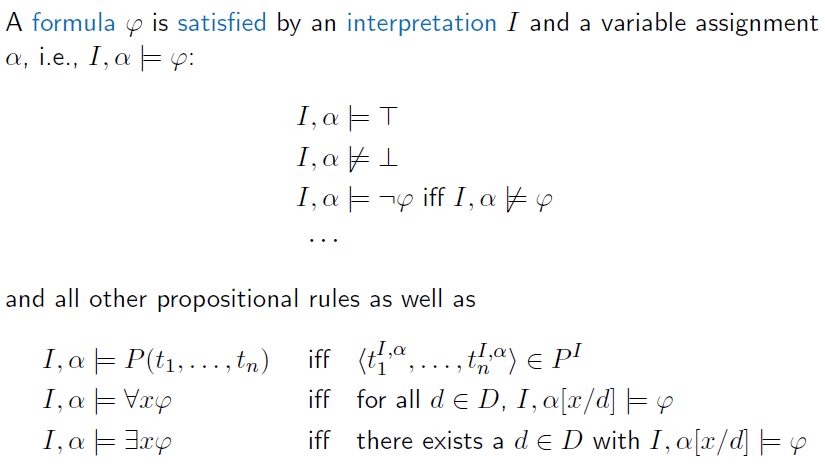
\includegraphics[scale=0.6]{45.png}
\subsection{Free and Bound Variables}

\includegraphics[scale=0.6]{46.png}\\
When boxed, is called \textit{free}, otherwis \textbf{bound}. Formulae with no free variables are called \textit{closed formulae} or \textit{sentences}.\\
With closed formulae, $\alpha$ can be left out on the left side of the model
relationship symbol: $I |= \omega$. An interpretation I is called a \textbf{model} of $\omega$ under $\alpha$ if: \textit{I,$\alpha|=\omega$}\\
\subsection{Derivation in PL1}
Reduction to propostional logic by instantiation based on the so-called \textbf{Herbrand Universe} (all possible terms) $->$ infinite propositional theories.\\
Simple way for special case: If the number of objects is \textbf{finite}, instantiate all variables by possible objects.\\
\subsubsection{Finite universes}
\textbf{Domain closure axiom }(DCA): $\forall[x=c_1 or .... or x=c_n]$\\
\textbf{unique name assumption/axiom or UNA}: $and_{i!=j}[c_i!=c_j]$\\
Eliminate quantification by instantiating all variables with all possible
values.\\
\subsubsection{Instantiation}
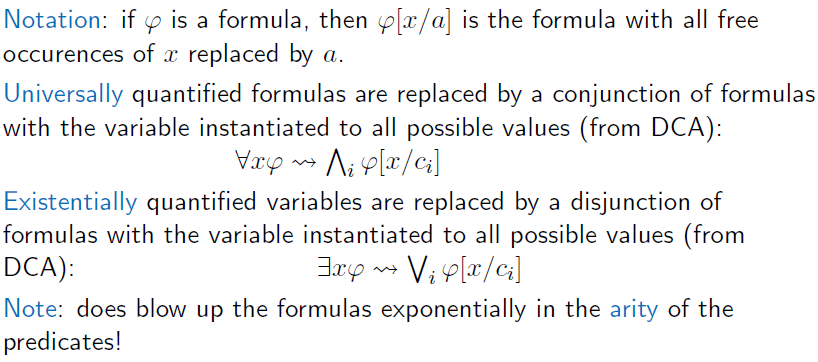
\includegraphics[scale=0.6]{47.png}

\section{Action Planning}
\begin{quote}
\textit{Planning is the art and practive of thinking before acting.\\\\
Planning is the process of generating (possibly partial) representations of future behavior prior to the use of such plans to constrain or control that behavior.}
\end{quote}
Planning is not searching, synthesis or scheduling.
\subsection{Planning Formalisms}
\subsubsection{Domain-Independent Action Planning}
\begin{itemize}
\item Start with a declarative specification of the planning problem
\item Use a domain-independent planning system to solve the planning problem
\item Domain-independent planners are generic problem solvers
\end{itemize}
\subsubsection{Planning as Logical Inference}
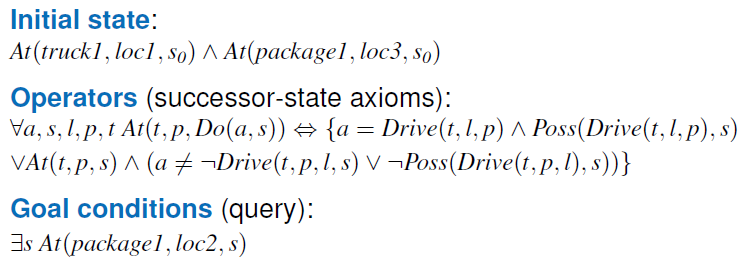
\includegraphics[scale=0.6]{48.png}\\
Inefficient for bigger sets.
\subsubsection{Basic STRIPS Formalism}
\textbf{STRIPS}: \textbf{ST}anford \textbf{R}esearch \textbf{I}nstitute \textbf{P}roblem \textbf{S}olver\\\\
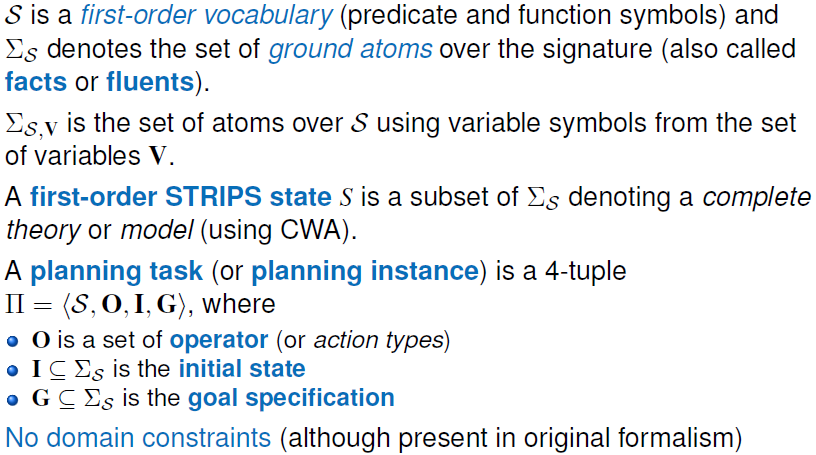
\includegraphics[scale=0.6]{49.png}\\\\
\begin{itemize}
\item \textbf{Operator: }o = <para,pre,eff>
\item \textbf{Operator instance or action: }operator with empty parameter list
\item \textbf{State change: }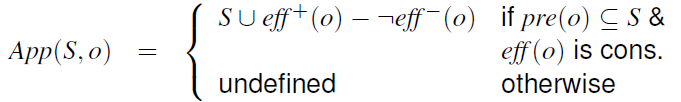
\includegraphics[scale=0.6]{50.png}
\end{itemize}
\includegraphics[scale=0.6]{51.png}\\\\
A plan $\Delta$ is a sequence of actions:\\
\includegraphics[scale=0.6]{52.png}\\
A plan is successful or solves a planning task if has a result that respects goal specifications.\\
\includegraphics[scale=0.6]{53.png}\\\\
STRIPS as described above allows for unrestricted first-order terms.\\
\textbf{Simplifications: }
\begin{itemize}
\item \textbf{1. Infinite state space: }No function terms (only 0-ary = constants).
\item \textbf{2. DATALOG-STRIPS: }No variables in operators (= actions).
\item \textbf{3. Propositional STRIPS: }used in planning algorithms nowadays.
\end{itemize}
\subsubsection{PDDL: The Planning Domain Description Language}
\begin{figure}
\includegraphics[scale=0.6]{54.png}
\caption{Logistics Example}
\end{figure}

\subsection{Basic Planning Algorithms}
We can view planning problems as searching for goal nodes in a large labeled graph (transition system). Nodes are defined by the value assignment to the fluents (states). Labeled edges are defined by actions. Create the transition system on the fly and visit only the parts that are necessary.\\
\includegraphics[scale=0.6]{55.png}\\\\

\begin{itemize}
\item \textbf{Progression Planning: Forward Search}
Start at initial state:\\
\textbf{1.} Initialize: $\Delta$ = $<>$, add the initial state and make it S.\\
\textbf{2.} Test whether we have reached goal: G in S? Return.\\
\textbf{3.} Select one applicable action \textit{$o_i$} non deterministically, compute successor S = App(S,$o_i$), extend plan adding it and \textbf{come back to step 2}.\\
This algorithm can be easily extended to more expressive planning languages (not only boolean: goal or not).\\ 
\includegraphics[scale=0.6]{56.png}\\\\

\item \textbf{Regression Planning: Backward Search}
Start from the goal:\\
\textbf{1.} Initialize: $\Delta$ = $<>$, add the goal state and make it S.\\
\textbf{2.} Test whether we have reached initial: I in S? Return.\\
\textbf{3.} Select one applicable action \textit{$o_i$} non deterministically which does not make sub-goals false, $S \cap \neg eff^-(o_i) = \emptyset$ and compute the regression of the description S through $o_i$:\\
\begin{center}
$S=S-eff^+(o_i)\cup pre(o_i)$
\end{center}
then extend plan $\Delta = <o_i,\Delta>$, back to step 2.\\
(Instead of non-deterministic we can use some search strategy).\\
\includegraphics[scale=0.6]{56.png}\\\\

\end{itemize}

\subsection{Computational Complexity}
\begin{itemize}
\item \textbf{Definition (Plan existence problem (PLANEX)): Does exist a plan that solve it?}
\item \textbf{Definition (Bounded plan existence problem (PLANLEN)): Doest there exist a plan of length \textit{n} or less that solves it?}
\end{itemize}
The state space for STRIPS with general first-order terms is infinite. The existence of a plan is then equivalent to the existence of a successful computation on the Turing machine. 
\begin{center}
\textbf{Theorem: }\textit{PLANEX for STRIPS with first-order terms is undecidable.}\\
\textbf{Theorem: }\textit{PLANEX is PSPACE-complete for propositional STRIPS.}
\end{center}
\textbf{- Restrictions on Plans}
If we restrict the length of the plans to be short, i.e., only polynomial in the size of the planning task, PLANEX becomes NP-complete. If we use a unary representation of the natural number k, then PLANLEN becomes NP-complete. We can use methods for NP-complete problems if we are only looking for “short” plans. 

\subsection{Current Algorithmic Approaches}
\begin{itemize}
\item \textbf{Heuristic Search Planning}: use an automatically generated heuristic estimator in order to select the next action or state. It is often easier to go for sub-optimal solutions (remember Logistics)
\item \textbf{Deriving Heuristics: Relaxations} Define a simplification (relaxation) of the problem and take the difficulty of a solution for the simplified problem as an heuristic estimator. (E.g.: Straight line distance on a map to estimate the travel distance).\\
\item \textbf{Ignoring Negative Effects: Example}\\
\includegraphics[scale=0.6]{57.png}
\end{itemize}


\section{Making simple decisions under uncertainty (Probability)}
In many cases, our knowledge of the world is incomplete (not enough information) or uncertain (sensors are unreliable). Without perfect knowledge, logical rules do not help much!\\
One possibility for expressing the degree of belief is to use probabilities. Probabilities quantify the uncertainty that stems from lack of knowledge.\\
\begin{center}
Decision Theory = Utility Theory + Probability Theory\\
$argmax_a \sum_{\omega} p(\omega|a)[U(\omega)-c(a)]$
\end{center}
\textbf{- Decision-Theoretic Agent}\\\\
\includegraphics[scale=0.6]{58.png}\\\\

\subsection{Foundations of Probability Theory}
We use random variables such as Weather (capitalized word), which has a domain of ordered values. In our case that could be sunny, rain, cloudy, snow (lower case words).\\
\begin{itemize}
\item \textbf{Unconditional Probabilities}: P(a) denotes the unconditional probability that it will turn out that A = \textit{true} in the absence of any other information.
\item P(a $|$ b) = $\frac{P(a \wedge b)}{P(b)} $is the conditional or posterior probability of a given that all we know is b: $P(cavity|toothace) = 0.8$\\
\textbf{- Product rule:} P($a \wedge b$)=P(a$|$b)P(b)\\
\end{itemize}
\subsection{Probabilistic Inference}
\subsubsection{Joint Probability}
The joint probability distribution P(X1,...,Xn) assigns a probability to
every atomic event. Example of such a complete instantiation:\\
\includegraphics[scale=1]{60.png}\\\\
All relevant probabilities can be computed using the joint probability by
expressing them as a disjunction of atomic events.\\
\includegraphics[scale=0.8]{61.png}\\\\
\textbf{- Total probability:} P(Y) = $\sum_z P(Y,z) = \sum_z P(Y|z)P(z)$\\\\
We can easily obtain all probabilities from the joint probability. The joint probability, however, involves kn values, if there are n random variables with k values.\\\\
\includegraphics[scale=0.8]{62.png}\\\\
In order to save memory and time, Modern systems work directly with conditional probabilities and make assumptions on the independence of variables (!conditional independence) to simplify calculations.\\

\subsubsection{Bayes' Rule}
Deriving from Product rule:\\
\begin{equation}
P(Y|X) = \frac{P(X|Y)P(Y)}{P(X)}
\end{equation}
Generalizing:\\
\begin{equation}
P(Y|X,e) = \frac{P(X|Y,e)P(Y|e)}{P(X|e)}
\end{equation}
\textbf{- Example:}\\
\includegraphics[scale=0.8]{63.png}\\\\
P(toothache $|$ cavity) (causal) is more robust than P(cavity $|$ toothache) (diagnostic).\\

\subsubsection{Relative Probability}
\includegraphics[scale=0.8]{64.png}\\\\

\subsubsection{Normalization}
To compute absolut probability of $P(c|t)$ without knowing P(t) we can do a complete case analysis using the property that $P(c|t)+P(\neg c|t) = 1$.\\
\includegraphics[scale=0.4]{65.png}\\\\
In general: $P(Y|X)= \alpha P(X|Y)P(Y)$\\\\
$\alpha$ is the normalization constant needed to make the entries in P($X|Y$) sum to 1 for each X. (e.g.: $\alpha(.1,.1,.3) = (.2,.2,.6)$)\\
\includegraphics[scale=0.4]{66.png}\\\\
\includegraphics[scale=0.4]{67.png}\\\\

\subsubsection{Multiple Evidence}
A probe by the dentist catches (Catch = true) in the aching tooth (Toothache = true) of a patient. We already know that P (cavity | toothache) = 0.8. Furthermore, using Bayes’ rule, we can calculate: \textbf{P (cavity | catch) = 0.95}\\
\includegraphics[scale=0.4]{68.png}\\
The dentist needs P ($tooth \wedge catch | cav$), i.e., diagnostic knowledge of all combinations of symptoms in the general case.\\
They are conditionally independent given that we know whether the tooth has a cavity:\\
$P(tooth|catch,cav) = P (tooth|cav)$\\
If one already knows that there is a cavity, then the additional knowledge of the probe catching does not change the probability.\\
$P (tooth \wedge catch | cav) = P (tooth | catch, cav)P (catch | cav) = \\
P (tooth | cav)P (catch | cav)$\\
The general definition of conditional independence of two variables X and Y given a third variable Z (a common cause) is:\\
$P(X,Y|Z)=P(X|Z)P(Y|Z)$\\

\subsubsection{Recursive Bayesian Updating}
Assuming conditional independence, multiple evidence can be reduced to prior probabilities and conditional probabilities. The general combination rule, if Z1 and Z2 are independent given X is $P(X | Z1 , Z2 ) = \alpha P(X)P(Z1 | X)P(Z2 | X) $where $\alpha$ is the normalization constant.\\
Generalization: $P(X|Z_1,...,Z_n)=\alpha P(X)/PI P(Z_i|X)$

\subsection{Bayesian Network}
Example of Burglary/Earthquake.\\\\
\textbf{- Domain knowledge/ assumptions:}\\
Events \textit{Burglary} and \textit{Earthquake} are independent. \textit{Alarm} might be activated by burglary or earthquake. \textit{John} calls if and only if he heard the alarm. His call probability is not
influenced by the fact, that there is an earthquake at the same time. Same for \textit{Mary}.\\
The \textit{random variables} are the \textit{nodes}. Directed edges between nodes represent \textbf{direct influence}. A \textbf{table of conditional probabilities (CPT) }is associated with every node, in which the effect of the parent nodes is quantified. The graph is acyclic (a \textbf{DAG}).\\
$P (maryCalls | alarm, burglary) = $\\
$P (maryCalls | alarm) and P (maryCalls | alarm, burglary, johnCalls, earthquake) $\\
$= P (maryCalls | alarm)$\\\\
$->$ Bayesian Networks can be considered as sets of (conditional) independence assumptions.\\
\textbf{- General formula: }\\\\
$P(x_1,...,x_n ) = P (x_n | x_{n-1},...,x_1 )\cdot ...\cdot P(x_2|x_1)P(x_1) =$\\
$\Pi_{i=1}^n P(x_i|x_{i-1},...,x_1)$\\
This is equivalent to:\\\\
$P(x_1,...,x_n) = \Pi_{i=1}^n P(x_i|parents(x_i))$\\
\includegraphics[scale=0.4]{69.png}\\
$P(j,m,a,¬b,¬e) = P(j|m,a,¬b,¬e)P(m|a,¬b,¬e)P(a|¬b,¬e)P(¬b|¬e)P(¬e)$\\
$=P(j|a)P(m|a)P(a|¬b,¬e)P(¬b)P(¬e)$\\
$= 0.9 × 0.7 × 0.001 × 0.999 × 0.998 = 0.00062$\\\\
In general, we need a table of size $2^n$ where \textit{n} is the number of variables. The size depends on the application domain (local vs. global
interaction) and the skill of the designer.\\
\textbf{- Naive Networks method :}\\
    - Order all variables\\
    - Take the first from those that remain\\
    - Assign all direct influences from nodes already in the network to the new node (Edges + CPT).\\
    - If there are still variables in the list, repeat from step 2.\\\\
\includegraphics[scale=0.4]{70.png} \\\\
\textbf{- Inference in Bayesian Network}\\
\includegraphics[scale=0.4]{71.png} \\\\
A node is conditionally independent of its non-descendants given its parents.\\
\textbf{- Example: }\\\\
\includegraphics[scale=0.3]{72.png}
\includegraphics[scale=0.3]{73.png}\\
\includegraphics[scale=0.3]{74.png}\\\\
Depth-first algorithm, linear space complexity, O($2^n$) time complexity.\\\\
\textbf{- Variable elimination: }\\
The algorithm can be improved by eliminating repeating or unnecessary calculations. The key idea is to evaluate expressions from right to left (bottom-up) and to save results for later use.\\\\
\includegraphics[scale=0.2]{75.png}\\
general observation: variables, that are not query or evidence variables and not ancestor nodes of query or evidence variables can be removed. Variable elimination repeatedly removes these variables and this way speeds up computation.\\
\textbf{within example: }Alarm and Earthquake are ancestor nodes of query
variable JohnCalls and cannot be removed. M aryCalls is neither a
query nor an evidence variable and no ancestor node. Therefore it can
be removed.\\\\
\textbf{- Complexity of exact inference: }\\
If the network is singly connected or a polytree, the time and space complexity of is linear.\\
For multiply connected networks inference in Bayesian Networks is
NP-hard.

\section{Acting under Uncertainty Maximizing Expected Utility}
\subsection{Introduction to Utility theory}

The utility function rates states and thus formalizes the desirability of a
state by the agent. A non-deterministic action A can lead to the outcome states  $Result_i(A)$. How high is the probability that the outcome state $Result_i(A)$ is reached,if A is executed in the current state with evidence E?\\
$→ P (Result i (A) | Do(A), E)$\\
\textbf{- Expected utility:}\\
$EU(A|E) = \Sigma_i P(Result_i(A)|Do(A),E) U(Result_i(A))$\\
The principle of \textbf{maximum expected utility (MEU)} says that a rational agent should choose an action that maximizes EU(A|E). \\
\textbf{- Problem: }Utility function requires search or planning, because an agent needs to know the possible future states in order to assess the worth of the current state (“effect of the state on the future”).\\

\subsection{Choosing Individual Actions}
\textbf{Preferences:}\\
$L_1 \succ L_2$ Agent prefers 1 over 2\\
$L_1 \sim L_2$ Agent is indifferent between 1 or 2\\
$L_1 \succsim L_2$ Agent prefers 1 or is indifferent.\\
\textbf{Orderability}\\
$(A \succ B) \lor (B \succ A)\lor(A \sim B)$\\\\
\textbf{Transitivity}\\
$(A\succ B)\lor(B\succ C) => (A \succ C)$\\\\
\textbf{Continuity}\\
$A\succ B \succ C => \exists p[p,A;1-p,C]\sim B$\\\\
\textbf{Substitutability}\\
$A\sim B \rightarrow [p,A;1-p,C]\sim [p,B;1-p,C]$\\\\
\textbf{Monotonicity}\\
$A\succ B=>(p > q \Leftrightarrow [p,A;1-p,B]\succ [q,A;1-q,B])$\\\\
\textbf{Decomposability}\\
$[p,A;1-p,[q,B;1-q,C]] \sim [p,A;(1-p)q,B;(1-p)(1-q),C]$\\\\
\textbf{Expected Utility of a Lottery:}\\
$U[p_1,S_1,...,p_n,S_n]) = \Sigma_i p_i U(S_i)$\\
Since the outcome of a nondeterministic action is a lottery, an agent can act rationally only by following the Maximum Expected Utility (MEU) principle.\\
Given a utility scale between $u_min$ and $u_max$ we can asses the utility of any
particular outcome S by asking the agent to choose between S and a standard lottery $[p,u_max;1-p,u_min]$. We adjust p until they are equally preferred.

\subsection{Sequential Decision Problems}
\includegraphics[scale=0.3]{77.png}\\\\
\begin{itemize}
    \item \textbf{Deterministic version:}\\
     All actions always lead to the next square in the selected direction, except that moving into a wall results in no change in position.\\
    \item \textbf{Stochastic version:}\\
     Each action achieves the intended effect with probability 0.8, but the rest of the time, the agent moves at right angles to the intended direction.
\end{itemize}

\subsection{Markov Decision Processes}
Stochastic environment defined by: States, Actions, Transition model P($s'|s,a$) (probability), Reward function R(s), Policy: mapping $\pi$ that specifies for each state which action to take. We, obviously, want the optimal policy $\pi*$ that maximizes the future expected reward.\\
Given the optimal policy, it executes the action $\pi^*(s)$. In this way we obtain a simple reflex agent.\\\\
\includegraphics[scale=0.5]{78.png}\\\\
\textbf{Performance} is measured by the sum of rewards. To determine the optimal policy, first calculate the utility of each state, it also depends on the horizon, if it is finite or infinite. For finite horizons the optimal policy is called nonstationary, instead for infinite it is stationary.\\

\textbf{- Stationary: }\\\\
Two ways to reward:\\
- Additive rewards: $U_h([s_0,s_1,...,s_n]) = R(s_0) + R(s_1)...$\\
- Discounted rewards: $U_h([s_0,s_1,...,s_n]) = R(s_0) + \gamma R(s_1)+ \gamma^2R(s_2)...$\\\\
$\gamma \in [0,1]$ is the discount factor. With discount, the utility is always finite. The discount factor expresses that future rewards have less than current rewards.

\subsection{Value Iteration}
$U^\pi(s)$ is the utility of a state under policy $\pi$. $s_t$ be the state of the agent after executing $\pi$ for t steps. The utility of s under $\pi$ is:\\
\begin{equation}
U^\pi(s) = E[\sum_{t=0}^\infty \gamma^tR(s_t)|\pi, s_0=s]
\end{equation}
R(s) is the short-term reward for being in s and U(s) is the long-term total reward from s onwards.\\\\
\includegraphics[scale=0.5]{79.png}\\\\
The agent simply chooses the action that maximizes the expected utility of the subsequent state:
\begin{equation}
\pi(s) = argmax_a\sum_{s'}P(s'|s,a)U(s')
\end{equation}
The utility of a state is the immediate reward for that state plus the expected discounted utility of the next state, \textbf{- Bellman-Equation}:
\begin{equation}
U(s) = R(s) + \gamma max_a \sum_{s'}P(s'|s,a)U(s')
\end{equation}
\textbf{- Example:}\\
\includegraphics[scale=0.5]{80.png}\\\\
\textbf{- Value Iteration}\\\\
An algorithm to calculate an optimal strategy. Basic Idea: Calculate the utility of each state. A sequence of actions generates a branch in the tree of possible states
(histories). A utility function on histories $U_h$ is separable iff there exists a function \textit{f} such that:\\
\begin{equation}
U_h([s_0,s_1,...,s_n])=f(s_0,U_h([s_1,...,s_n]))
\end{equation}
The simplest form is an additive reward function R:
\begin{equation}
U_h([s_0,s_1,...,s_n])=R(s_0)+U_h([s_1,...,s_n])
\end{equation}
Typical problems contain cycles, which means the length of the histories is potentially infinite.Solution: Use
\begin{equation}
U_{t+1}(s) = R(s) + \gamma max_a \sum_{s'}P(s'|s,a)U_t(s')
\end{equation}
The Bellman equation is the basis of value iteration, thanks to the max-operator the n equations for the n states are nonlinear. We can apply an iterative approach in which we replace the equality by an assignment:
\begin{equation}
U(s') \leftarrow R(s) + \gamma max_a \sum_{s'}P(s'|s,a)U(s')
\end{equation}
\textbf{- Algorithm}\\\\
\includegraphics[scale=0.5]{81.png}\\\\
\textbf{- Convergence:}\\\\
\includegraphics[scale=0.5]{82.png}\\\\

\subsubsection{Policy Iteration}
Policy iteration alternates the following two steps beginning with an initial policy $\pi_0$ :
\begin{itemize}
\item \textbf{Policy evaluation: } given $\pi_t$, calculate $U_t=U^{\pi t}$ the utility if $\pi_t$ was executed.
\item \textbf{Policy improvement: }calculate a new maximum expected utility policy $\pi_{t+1}$ according to:
\begin{equation}
\pi_{t+1}(s)=argmax_a\sum_{s'}P(s'|s,a)U_t(s')
\end{equation}
\end{itemize}
\includegraphics[scale=0.5]{83.png}\\\\

\section{Machine Learning}
An agent learns when it improves its performance w.r.t. a specific task with experience.\\
\subsection{The learning agent}
\textbf{Performance element: }Processes percepts and chooses actions.\\
\textbf{Learning element: }Carries out improvements.\\
\textbf{Critic: }Evaluation of the agent’s behavior based on a given external behavioral measure.\\
\textbf{Problem generator: }Suggests explorative actions that lead the agent to new experiences.\\\\
\subsection{Types of learning}
\textbf{Supervised learning:} Involves learning a function from examples of its inputs and outputs.\\
An example is a pair (x, f (x)). The complete set of examples is called the \textbf{training set.} Pure inductive inference: for a collection of examples for f, return a function h (hypothesis) that approximates f.
A good hypothesis should predict unseen examples correctly. A \textbf{hypothesis is consistent} with the data set if it agrees with all the data.
\textbf{Ockham’s razor: }prefer the simplest hypothesis consistent with the data.\\\\

\textbf{Unsupervised learning: }The agent has to learn patterns in the input when no specific output values are given.\\\\
\textbf{Reinforcement learning: }The most general form of learning in which the agent is not told what to do by a teacher. Rather it must learn from a reinforcement or reward. It typically involves learning how the environment works.\\

\subsection{Decision trees}

\textbf{Input:} set of attributes.\\
\textbf{Output:} a decision.\\
Continuous (regression) or discrete (classification), binary or not.

\subsubsection{Boolean Decision Trees}
\textbf{Input: }set of vectors of input attributes.\\
\textbf{Output: }Yes/No decision based on a goal predicate.\\
\textbf{Properties:  }an internal node represents a test of a property, branches are labeled with the possible values, each leaf specifies the returning value.\\\\
\textbf{Example: }\\\\
\includegraphics[scale=0.3]{84.png}\\\\
Each decision tree hypothesis can be seen as an assertion of the form:
\begin{equation}
\forall s WillWait(s)\leftrightarrow (P_1(s)\vee P_2(s)\vee ... P_n(s))
\end{equation}
$P_i(s)$ are the tests along the path. \textbf{Limitation:} trees always involve just one variable.\\\\
\textbf{Compact representations: }\\\\
We can construct a decision tree by translating every row of a truth table to a path in the tree. This can lead to exponential trees (parity, majority).\\\\
\textbf{- Training Set example:}\\\\
\includegraphics[scale=0.3]{85.png}\\\\
\textbf{- Creation possibilities: }\\
\begin{itemize}
\item \textbf{Naive: }simply construct with one path to a leaf for each example. Test all attributes. Even if it will classify the examples, It will not say anything about other classes. It just memorizes the observation and doesn't generalize.
\item \textbf{Smallest solution: } Applying Ockham's razor we find the smallest decision tree. unfortunately, the smallest definition is intractable.
\item \textbf{Divide and Conquer: }Choose an attribute, Split the training set such that each corresponds to a particular value of that attribute, recursive apply this process to the smaller sets.\\
\includegraphics[scale=0.3]{86.png}\includegraphics[scale=0.3]{87.png}\\\\
Type is a poor attribute since it leaves us with state full of true and false.\\
Patrons is a better choice.\\\\
In each recursive step there are 4 cases:\\
\begin{itemize}
\item \textbf{Positive and negative: }choose a new attribute.
\item \textbf{Only positive: }finished.
\item \textbf{No examples: }Answer the majority
\item \textbf{No attributes left: }Too noisy.
\end{itemize}
\includegraphics[scale=0.3]{88.png}
\includegraphics[scale=0.2]{89.png}\\\\
\end{itemize}
\textbf{- Properties of the Resulting tree:}\\
The learning algorithm outputs a tree that is consistent with all examples it has seen.\\
The tree does not necessarily agree with the correct function. Some tests (Raining, Reservation) are not included (are useless) since the algorithm can classify the examples without them.\\\\
\textbf{- Choosing Attribute Tests}\\
One goal of decision tree learning is to select attributes that minimize the depth of the final tree. The \textbf{perfect attribute }divides the examples into sets that are all positive or all negative. Patrons is not perfect but fairly good. Type is useless since the resulting proportion of positive and negative examples in the resulting sets are the same as in the original set.\\\\
\textbf{- Information provided by an Attribute}\\
One suitable measure is the expected amount of information provided by the attribute.\\
In general, if the possible answers $v_i$ have probabilities $P(v_i)$, the information content is given as the entropy:\\
\begin{center}
$I(P(v_1),...,P(v_n)) = \sum_{i=1}^n -P(v_i)log_2(P(v_i))$
\end{center}
\includegraphics[scale=0.3]{90.png}\\\\
\textbf{- Attribute Selection}\\
The value of an attribute A depends on the additional information that we still need to collect after we selected it. A random example has value i with probability: $\frac{p_i+n_i}{p+n}$.\\
\textbf{The average information content after choosing A is: }$R(A) = \sum_{i=1}^v \frac{p_i+n_i}{p+n}I(\frac{p_i}{p_i+n_i},\frac{n_i}{p_i+n_i})$\\
\textbf{The information gain from choosing A is: }$Gain(A) = I(\frac{p}{p+n},\frac{n}{p+n})-R(A)$.\\
Heuristic in Choose-Attribute is to select the \textit{attribute with the largest gain.}\\
\includegraphics[scale=0.3]{91.png}\\\\
\textbf{The training and test sets must be kept separate.}\\

\section{Deep Learning}
\subsection{Why?}
Excellent empirical results in a lot of Learning fields. Learning as an Alternative to Traditional Programming, we don’t understand how the human brain solves certain problems, we can nevertheless learn these tasks from data/experience. If the task changes, we simply re-train. We can construct computer systems that are too complex for us to understand anymore ourselves. Learning from data / experience may be more human-like.
\subsection{Representation Learning and Deep Learning}
\textbf{- Representation Learning: }a set of methods that allows a machine to be fed with raw data and to automatically discover the representations needed for detection or classification.\\
\textbf{- Deep Learning: }representation learning methods with multiple levels of representation,composing nonlinear modules.\\
\textbf{- ML Pipeline: }high-level attributes or features of the data E.g., the binary attributes we used for decisions trees (feature engineering).\\
\textbf{- RL Pipeline: }Jointly learn features and classifier, directly from raw data
This is also referrred to as end-to-end learning.\\\\
ANNs are inspired by biology: Dendrites input information to the cell, Neuron fires (has action potential) if a certain threshold for the voltage is exceeded, Output of information by axon, The axon is connected to dentrites of other cells via synapses.\\\\
The advance doesn’t depend only on the computer power, but also on the methodological improvements.
\subsection{Multilayer Perceptrons}
\includegraphics[scale=0.3]{92.png}\\\\
\textbf{Linear funciton of previous layer's outputs: }$z_{k-1}:a_k = W_k\cdot z_{k-1}+b_k$\\
\textbf{Nonlinear transformation: }$z_k = h_k(a_k)$\\\\
\includegraphics[scale=0.3]{93.png}\includegraphics[scale=0.3]{94.png}\\\\
\textbf{- For regression: }single output with linear activation, loss function is squared error:
\begin{center}
$L(w)=\frac{1}{2}\sum_{n=1}^N{y^^(x_n,w)-y_n}^2$
\end{center}
$x_n$ is the raw input, $y_n$ is the true value of data point.\\
\textbf{- For classification: }single output with logistic activation and loss function is negative log likelihood (\textit{cross-entropy}):
\begin{center}
$L(w)=-\sum_{n=1}^N{y_n\ln y^^ +(1-y_n)ln(1-y^^ _n)}$
\end{center}
To \textbf{optimize a loss function} usually the weights are adapted to minimize the error, one technique can be using gradient-based optimization: gradients are computed and use of backpropagation using small batches of the data$\rightarrow$ \textbf{Stochastic gradient descent (SGD)}.\\
\textbf{- Convolutions: } Start from a 3D image dot producted for a smaller 3D filter: $w^Tx+b$\\
Based on the filter, the convolution layer is divided in activation maps.\\\\
\includegraphics[scale=0.3]{95.png}\\\\
The second one is a \textbf{Recurrent Neural Networks: }cycles let information persist in the network for some time (state), and provide a time-context. Implement dynamical systems. Turing complete.
\subsection{Reinforcement Learning}
Finding optimal policies for MDPs composed of: states, actions, transition model and rewards. Policy: complete mapping $\pi$ that specifies for every state s which action to take.\\\\
\includegraphics[scale=0.3]{96.png}
\subsection{Limitations}
All we've seen till now is bottom-up, there is no logic and no reasoning. It's very far from human performance.\\\\
\includegraphics[scale=0.3]{97.png}\\\\
\textbf{- So why Deep Learning?}\\
Excellent empirical results in many domains and very scalable, similar to human reasoning, allows end-to end learning.

\section{Natural Language Processing}
\subsection{Motivations and Tasks}
NLP creates interfaces between human language and computers.\\
\textbf{Goal:} automatic processing of large amounts of human language data,\\
Traditional rule-based approaches and (to a lesser degree) probabilistic NLP models faced limitations as human errors, rules and labels.
\subsection{Learning Representations}
\textbf{- Word Embedding: }mapping function from words to $R^n$. It realizes a look-up table such that related words are near and unrelated words have great distance.\\
A word embedding function W can be trained using different tasks. EX.: predict, if a 5-gram (sequence of five words) is valid or not.\\
Training data contains valid and slightly modified, invalid 5-gramsTrain the combination of embedding function W and classification module R.\\
Embedding allows to work not only with synonyms, but also with other words of the same category. In the embedding space, systematic shifts can be observed for analogies.\\
\textbf{- Bilingual Word Embedding: } train two embeddings in parallel such, that corresponding words are projected to close-by positions in the word space.
\subsection{Sequence-to-Sequence Deep Learning}
\subsubsection{Association Modules}
Limitation on number of input words can be overcome by adding association modules, which can combine two word and phrase representations and merge them.\\\\
\includegraphics[scale=0.3]{98.png}\\\\
\subsubsection{From Representations to the Translation of Texts}
For translations, we also need disassociation modules (encoder - decoder principle)\\\\
\includegraphics[scale=0.3]{99.png}\\\\
Take context into account by learning the importance of neighboring words $\rightarrow$ attention mechanism. The same principle is used for voice recognition but here we take into account Frequency and time.














































\end{document}
